\documentclass[11pt,a4paper]{article}
% Shared look for Laile's submission documents. Build with Tectonic (see submission/build.sh).
\usepackage{fontspec}
\usepackage{xcolor}
\usepackage{graphicx}
\usepackage{tikz}
\usetikzlibrary{positioning,fit,backgrounds,arrows.meta,calc,shapes.misc}

% macOS system fonts: Avenir Next for text, Hiragino Sans GB for 莱乐.
\setmainfont{Avenir Next.ttc}[
  Path=/System/Library/Fonts/,
  UprightFeatures={FontIndex=7},
  BoldFont={Avenir Next.ttc}, BoldFeatures={FontIndex=2},
  ItalicFont={Avenir Next.ttc}, ItalicFeatures={FontIndex=4},
  BoldItalicFont={Avenir Next.ttc}, BoldItalicFeatures={FontIndex=3}]
\setsansfont{Avenir Next.ttc}[
  Path=/System/Library/Fonts/,
  UprightFeatures={FontIndex=7},
  BoldFont={Avenir Next.ttc}, BoldFeatures={FontIndex=2},
  ItalicFont={Avenir Next.ttc}, ItalicFeatures={FontIndex=4},
  BoldItalicFont={Avenir Next.ttc}, BoldItalicFeatures={FontIndex=3}]
\newfontfamily\heavyfont{Avenir Next.ttc}[Path=/System/Library/Fonts/, UprightFeatures={FontIndex=8}]
\newfontfamily\cjk{Hiragino Sans GB.ttc}[Path=/System/Library/Fonts/, UprightFeatures={FontIndex=2}]

% The app's palette (DesignSystem/Theme.swift).
\definecolor{accent}{HTML}{0F8A6A}
\definecolor{accentsoft}{HTML}{DFF3EC}
\definecolor{reward}{HTML}{E8930C}
\definecolor{rewardsoft}{HTML}{FFF1DC}
\definecolor{danger}{HTML}{C62828}
\definecolor{dangersoft}{HTML}{FDE7E5}
\definecolor{ink}{HTML}{17211C}
\definecolor{muted}{HTML}{5D6B63}
\definecolor{surface}{HTML}{EEF2EF}
\definecolor{paper}{HTML}{F6F7F5}

\newcommand{\laile}{Laile ({\cjk 莱乐})}
\newcommand{\lele}{Lele ({\cjk 乐乐})}
\newcommand{\wordmark}{{\cjk\color{accent}莱乐}}

\usepackage[a4paper,margin=1.8cm]{geometry}
\usepackage[hidelinks]{hyperref}
\usepackage{enumitem}
\usepackage{caption}
\setlength{\parindent}{0pt}
\setlength{\parskip}{6pt}
\setlist{nosep, leftmargin=1.2em, topsep=2pt}
\captionsetup{font={small,color=muted}, labelfont=bf, skip=4pt}
\setlength{\fboxsep}{0pt}\setlength{\fboxrule}{0.4pt}
\pagestyle{empty}
\color{ink}

\newcommand{\shot}[2]{\begin{minipage}[t]{0.48\linewidth}\centering
  \fbox{\includegraphics[width=\linewidth]{#1}}\\[3pt]{\small\color{muted}#2}\end{minipage}}

\begin{document}

{\fontsize{22}{26}\selectfont\bfseries Laile: CodeBuddy, WorkBuddy and Miora history}\\[4pt]
{\color{muted}Charles Andrew Lim \textbullet\ Tencent Cloud AI CAN DO IT Hackathon Singapore 2026\\\href{https://github.com/LimCharles/laile}{github.com/LimCharles/laile}}

{\color{accent}\rule{\linewidth}{1.2pt}}

\textbf{WorkBuddy (CodeBuddy's coding agent, Tencent Hy4)} worked on the Laile repository through its GitHub connector. It cloned the code, ported the safety rules to Python to try real phrasings against them, and later installed a Swift toolchain to build and test its own changes.
\begin{itemize}
  \item \textbf{Safety audit} of the symptom rules. It found that a denial of pain hid numbness (``no pain but my foot is numb'' got ``carry on''), that ``no chest pain'' raised a false emergency, that a pain threshold could become 11 on a 0 to 10 scale, and that a stop decision during rest was ignored.
  \item \textbf{Safety fixes.} It implemented the six fixes with tests for every case in its audit: 112 core tests passing, up from 92. The commit was reviewed and merged, followed by a review commit that keeps ordinary workout talk (``my heart is racing'') from raising red flags.
  \item \textbf{ADP integration review.} Sixteen findings on Lele's ADP calls, the most serious being that ``I haven't taken it yet'' was logged as a taken dose. The confirmed findings were fixed with regression tests.
\end{itemize}
\textbf{Miora} made the brand from one brief with its Brand Specialist skill (logo, cover, app icon and the Lele mascot), and later the title cards, scene backgrounds and Lele poses for the demo video.

\vspace{6pt}
\begin{center}
\shot{01-safety-audit-request.jpg}{1. Asking WorkBuddy for a safety audit}\hfill
\shot{02-safety-audit-findings.jpg}{2. Its findings, with files and lines}
\end{center}

\newpage
\begin{center}
\shot{03-safety-audit-coverage.jpg}{3. Coverage: phrasings the rules missed}\hfill
\shot{06-safety-fixes-done.jpg}{4. The six fixes, with tests passing}\\[14pt]
\shot{04-adp-review-request.jpg}{5. Asking for a review of the ADP integration}\hfill
\shot{05-adp-review-findings.jpg}{6. The review's findings}
\end{center}

\newpage
\begin{center}
\shot{07-miora-brand-chat.jpg}{7. Miora: the brand brief and its answer}\hfill
\shot{08-miora-brand-canvas.jpg}{8. Miora: logo, cover, app icon and Lele}\\[14pt]
\begin{minipage}[t]{0.75\linewidth}\centering
  \fbox{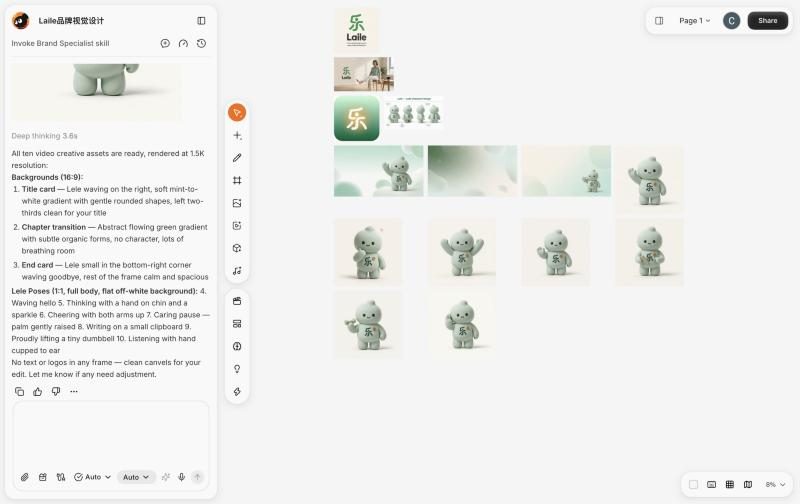
\includegraphics[width=\linewidth]{09-miora-video-creatives.jpg}}\\[3pt]{\small\color{muted}9. Miora: title cards, scene backgrounds and seven Lele poses for the demo video}
\end{minipage}
\end{center}

\end{document}
